\chapter{Introduction}
\pagenumbering{arabic}
\label{c:intro}
    Advances in 3D scanning technology and 3D modeling
    techniques have lowered the barrier in creating
    high-resolution 3D models.  
    High-resolution 3D models can now be created
    with laser scanner and reconstruction software.
    For example, the Stanford's Digital Michelangelo Project
    has digitalized several famous statues of Michelangelo
    \cite{levoy00digital} (See Figure \ref{f:intro:scanner}). 
    Similar projects include 
\begin{figure}[htbp!]
\centering
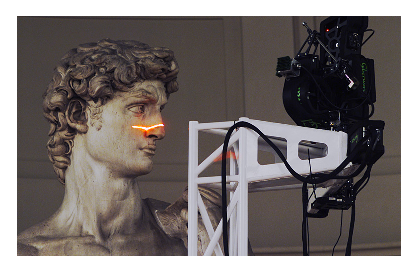
\epsfig{file=scanner.eps, width=0.6\textwidth}
\caption[Stanford's Digital Michelangelo Project.]{Stanford's Digital Michelangelo Project. The head of David Statue is being 
scanned (image source: http://graphics.stanford.edu/projects/mich).}\label{f:intro:scanner}
\end{figure}
    the Digital Sculpture Project \cite{deroos2004dsp}
    and the project to digitize Rodin's sculptures \cite{miyazaki2006dab}. 
    Further, artists can directly create high-resolution 3D models with
    digital sculpture softwares such as ZBrush (See Figure \ref{f:intro:zbrush}).
\begin{figure}[htbp!]
\centering
\begin{tabular}{cc}
\epsfig{file=zbrush1.eps, height=0.33\textwidth}
&
\epsfig{file=zbrush2.eps, height=0.33\textwidth}
\end{tabular}
\caption[Complex digital sculptures created with ZBrush.]{Complex digital sculptures created with ZBrush
(image source: http://www.evermotion.org/vbulletin/showthread.php?t=64128).}\label{f:intro:zbrush}
\end{figure}

    Sharing high-resolution 3D models over the Internet is useful in many
    applications. Digital museum exhibiting 3D models of artifacts
    is one of the applications. For example, Dr. Andre Stork and his teams are working
    on a project named ``History in 3D''\footnote{
    http://www.fraunhofer.de/en/press/research-news/2009/11/history-in-3d.jsp.}. 
    Exhibiting high-resolution 3D models of artifacts instead of the
    artifacts themselves has many advantages. 
    People can view the artifacts from
    anywhere, at anytime, and without any travel cost. 
    Visitors can interact with exhibited artifacts
    in any way they want, without worrying about damaging them 
    or interfering other visitors. 
    Moreover, the museum can exhibit artifacts, however precious they are, 
    safely without worrying about corrosion and theft.


    High-resolution 3D models are useful in other networked applications too. 
    For example, virtual world applications,
    such as Second Life, can become more realistic and interesting by
    supporting high-resolution 3D models. 
    Commercial users could show their products as 3D models to potential users all over 
    the world. Sculptors could demonstrate their artworks freely without renting a gallery.
    As another example, virtual earth applications, 
    such as Google Earth, could represent many landmark buildings or statues
    (e.g. Statue of Liberty) as high-resolution 3D models to
    give more realistic representation of the real world.

    When used in networked applications, 
    high resolution 3D models may take a long time to download completely
    for display at the client. 
    For example, the Stanford model of the David statue, with 28 million vertices and
    56 million triangles, is still 70 MB in size with
    state-of-the-art compression \cite{alliez2001progressive} and needs around 10 minutes
    to download at 1 Mbps.  
    To reduce the waiting time of the user, 
    streaming techniques can be used to transmit 3D models. 
    The 3D streaming technology enables users to render a coarse version of the model
    based on partially received data as a preview, 
    and then improve the quality when more data becomes available. 
    Users can decide how much data to receive based on their requirement of quality
    and the rendering ability of their hardware.

\begin{figure}[htbp!]
\centering
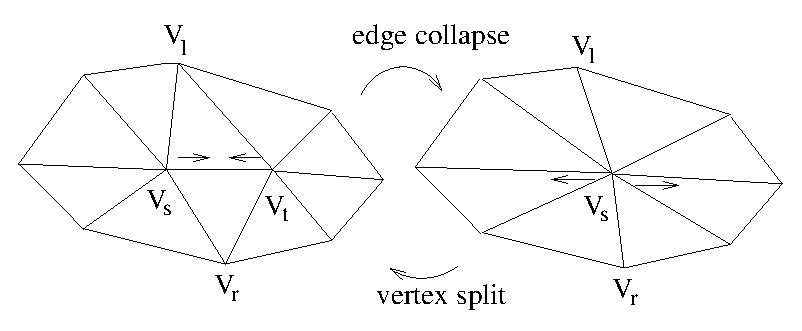
\epsfig{file=split2.eps, width=0.5\textwidth}
\caption{Edge collapse and vertex split}\label{f:intro:split2}
\end{figure}
    One popular representation to support 3D streaming, \textit{progressive mesh}, 
    is proposed by Hoppe \cite{hoppe96progressive}.
    The technique is based on an
    operation called \textit{edge collapse}, and its reverse
    operation, \textit{vertex split}.  Given a (non-progressive)
    3D mesh, the technique applies a series of edge collapses,
    simplifying the model by reducing the number of vertices and
    faces.  The final, simplified model obtained after this
    process becomes the \textit{base model}.  Given a base model,
    we can reconstruct the original model by reversing
    the edge collapse operations through \textit{vertex splits},
    incrementally adding new vertices and faces. So, a
    progressive mesh can be represented by the base
    model and a series of vertex splits.  
    Figure~\ref{f:intro:split2} illustrates edge
    collapse and vertex split operations.
    Progressive streaming can be implemented by sending the base mesh
    first as a preview and then sending vertex splits to improve 
    the quality incrementally (See Figure \ref{f:intro:progressive}).
    \begin{figure}[htbp!]
    \centering
    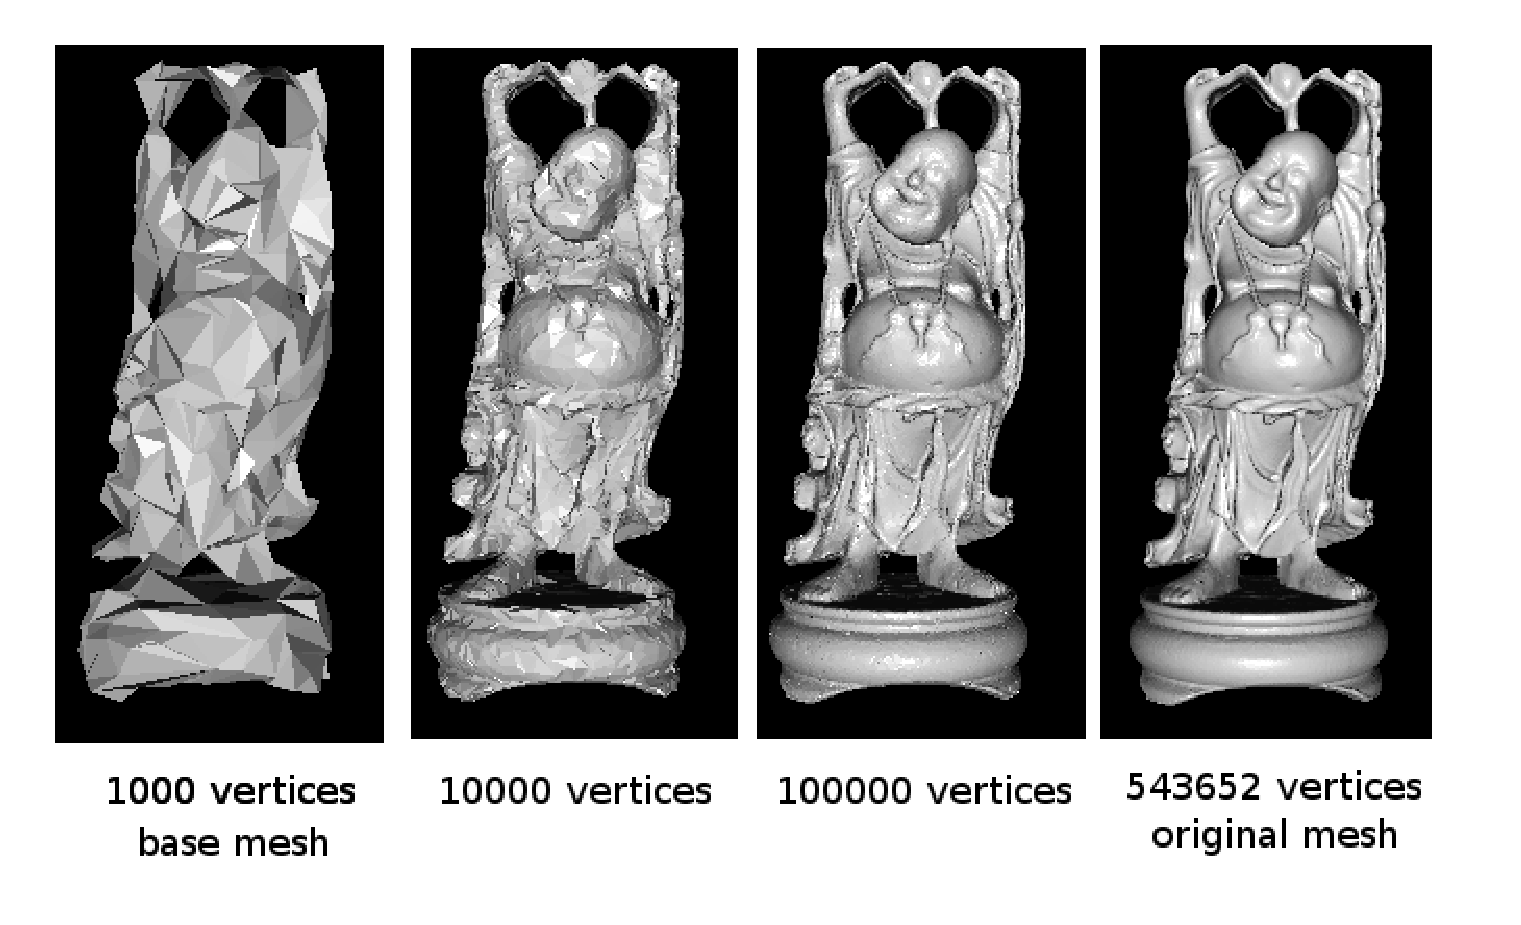
\epsfig{file=progressive.eps, width=0.85\textwidth}
    \caption[Progressive 3D mesh streaming.]{
    Progressive 3D mesh streaming. The original Happy Buddha mesh 
    courtesy of Stanford Computer Graphics Laboratory.
    \label{f:intro:progressive}}
    \end{figure}
    
    Although audio and video streaming have been studied extensively, 
    3D streaming remains a new research topic. 
    Video streaming and 3D streaming are significantly different
    due to the difference between videos and 3D models, and
    the main difference is how users consume the data.
    In video streaming, usually the data are consumed in time order. 
    Whereas in 3D streaming, especially when high-resolution 3D models are used,
    users may consume different subset of the data in various orders.
    
    This flexibility is important in streaming of high-resolution 3D models, 
    because streaming a huge 3D model in a fixed order leads to transmission of data not
    useful to the user, wasting time and bandwidth.
    Ensuring this flexibility in streaming systems is an important consideration
    in choosing representation and coding schemes. The details are discussed
    in Chapter \ref{c:related}.
    Meanwhile, this flexibility introduces some new research questions, 
    which we introduce in the next section. 

  \section{Research Objectives and Scope}
  \label{s:intro:objectives}
    \subsection{Quantitatively Determining the Effect of Dependency}
    In progressive streaming, the quality of the mesh on the receiver
    increases over time.
    Because vertex splits contribute differently to the quality, 
    how quality improves
    depends on the decoding order of the vertex splits,
    which in turn depends on the sending order of the vertex splits.
    Because of the flexibility in choosing sending order,
    it is possible to choose a sending order so that the 
    quality on the receiver increases as fast as possible.

    A natural method is to send vertex splits in the descending order
    of their contribution to the quality of the received mesh. 
    This strategy, however, is not always optimal 
    when the mesh is transmitted over a lossy network,
    because dependency also plays an important role in choosing sending order.
    
    The progressive coding of meshes introduces dependencies among 
    the vertex splits, and the descendants cannot be decoded
    before their ancestors are all decoded. Therefore, 
    when a progressive mesh is transmitted over a lossy network,
    a packet loss will delay the decoding of the following
    vertex splits if they depend on this lost packet. 
    These successfully received vertex splits cannot be 
    decoded until the lost packet is successfully retransmitted. 
    Hence, another consideration in choosing sending order
    is to minimize the dependency among packets so that most
    received vertex splits can be decoded without waiting.
    
    Therefore, to choose a proper sending order, it is essential 
    to find a proper trade-off between the importance of vertex
    and the dependency among packets. Understanding the trade-off
    requires us to quantify the effect of dependency, 
    which is is non-trivial, as
    the effect depends on which packets are lost during transmission.
    Packet losses are random, so the effect of dependency  
    can only be estimated probabilistically.
    
    In summary, the first research objective in this thesis is
    \textit{to quantitatively analyze the effect of dependency on 
    the quality of reconstructed progressive meshes 
    during transmission over lossy network, and to find
    a proper sending order to improve the quality as quick
    as possible, considering both the importance of vertex splits
    and dependency among the vertex splits.}
    
    \subsection{Receiver-Driven View-Dependent Streaming System of Progressive Meshes}
    Another factor, the viewpoint of the user, 
    needs to be considered in deciding the sending order of vertex splits.
    Sending non-visible data before visible data wastes bandwidth
    that could be used to send more visible data. 
    Moreover, the visual contributions of visible
    vertex splits (how much they can improve the rendered image)
    also depend on the viewpoint of the user.
    Hence, deciding which vertex splits to send (and in what order)
    according to the viewpoint of the user, 
    so called \emph{view-dependent streaming}, 
    is crucial to improve the rendered quality of the mesh.
    
    In existing solutions to view-dependent streaming,  
    the sender decides the sending order. 
    This sender-driven protocol has several drawbacks. 
    First, it is not scalable to many receivers as the sender has to
    determine the visibility of vertices for each receiver. 
    Second, the sender needs to maintain
    the state of each receiver to avoid sending duplicate data. 
    Due to the stateful design and high computational requirements,
    the sender-driven approach cannot be easily extended to support 
    many receivers with caching proxy and peer-to-peer system,
    two common solutions to scalability. 

    To address the drawbacks of the sender-driven protocol, we want
    to design a stateless sender for scalable view-dependent progressive 
    mesh streaming, in which the sending order is decided by the receiver.
    We call this approach the \textit{receiver-driven} approach.
    
    To design a receiver-driven view-dependent mesh streaming
    system is challenging. The most important
    challenge is how the receiver determines the visibility and visual contribution
    of vertex splits before receiving them. The receiver does not have
    the complete data, unlike the sender. The receiver thus has to estimate
    the visibility and visual contribution of vertex splits based on 
    partially received data. Moreover, the sender, being stateless, increases
    the difficulty in compressing data, because now the sender is not aware
    of the sending order of the vertex splits, and most existing compression algorithms
    are not applicable since they require specific sending orders.
    As a result, we need to find an efficient 
    compression algorithm which does not rely on the sending order.

    In summary, the second objective in this thesis is 
            \textit{to design and implement
            a receiver-driven view-dependent streaming system, where
            the visibility and the sending order are decided by the receiver instead of the sender,
            thus making the sender stateless and improving the scalability of the system.}

            \begin{comment}
    \subsection{Patterns of User Behaviors in Viewing 3D Meshes}
    In a view-dependent steaming system, the sending order and sending subset 
    of data highly depend on the interactivity of users. 
    Designing a satisfying system
    requires an understanding of user behaviors in viewing 3D meshes.
    For example, if user actions are somewhat predictable, pre-fetching can 
    be used to reduce the response time. If we know in advance that some parts
    of a huge mesh are requested more frequently, they can be 
    cached to significantly reduce server overhead.

    Moreover, by deriving certain pattern in users' interaction with
    high-resolution meshes, we can generate a large number of synthetic traces,
    which simulate users' actions, to be used in measuring system
    performance during simulations. This method is much cheaper than collecting 
    a large number of traces from real users and can be used in developing and evaluating
    prototypes. 

    The first step of understanding user behaviors is to collect the traces of 
    how user interact with the high-resolution 3D models. Because there are no
    existing popular applications, we implement our own application and
    design the data collecting process.
    After collecting the user traces, we need to develop proper methods to analyze
    the traces and derive some patterns. This task is challenging because of the high
    flexibility in users' interaction. Users can move the mesh freely in 3D space, and
    there are six degree of freedom. Moreover, the time they stay in a position is arbitrary
    and users can leave the system at any time. All these flexibilities could make the traces
    extremely diversified.
    
    Most previous work on user interactions with 3D objects focused on design
    of specific interaction techniques (e.g., the study by Chen et al. \cite{chen88study}
    and Hinckley et al. \cite{hinckley97usability}). 
    As far as we know, there is no study before us that study user behavior
    from the system design point of view.
    
    Therefore, the third objective of this thesis is 
    \textit{
            to study user behavior from the system design point of view, 
            such as predictability and access patterns (for caching), and
            find a model to generate synthetic traces to simulate user behaviors.
            }
        \end{comment}

    \subsection{P2P View-Dependent Progressive Mesh Streaming System}
    The receiver-driven protocol significantly reduces the computing cost at the sender,
    but the bandwidth can remain the bottleneck if each receiver receives data
    from the same sender and the number of receivers becomes large. 
    Peer-to-peer (P2P) technique is a common solution to increase
    the scalability without incurring high infrastructural cost. 
    As a result, applying P2P technique in a view-dependent mesh steaming
    system enables small companies and individual users to publish
    their high-resolution 3D models. Hence, P2P technique is essential
    to popularize applications using high-resolution 3D models.
    
    Applying P2P techniques into progressive mesh streaming system
    is considerably simplified by our receiver-driven protocol since 
    the sender is stateless and free of expensive computations.
    The implementation is still challenging due to the flexibility
    in choosing the sending order and subset to send.
    
    In P2P mesh streaming, users 
    may choose to look at different facets or zoom into different level.
    Therefore, each peer may choose a unique sending order of
    vertex splits. Hence, how to group vertex splits into chunks (the data unit
    for user sharing) is not straightforward. 
    Moreover, since peers may download different subsets of the
    mesh, it is difficult for a peer to keep receiving
    needed data from the same peer.  
    A peer would have to continuously look for peers to retrieve the mesh data from, 
    which makes content discovery more challenging.

    In summary, the last objective of this thesis is 
    \textit{
            to investigate chunking and content discovery problems introduced by 
            the flexibility in choosing sending order and sending subset, and
            to implement a prototype of P2P view-dependent mesh streaming system
            based on the receiver-driven protocol proposed in this thesis.
            }
    
    \subsection{Scope}
            The scope of our research is as follows.

            First, only streaming of static 3D objects is considered in this thesis. 
            Streaming of 3D animations is beyond the scope of this thesis. 
            Second, streaming of 3D scenes is not concerned in this thesis.
            Instead, this thesis concentrates on streaming of a single large mesh.
            Nonetheless, streaming of 3D scenes becomes easier when mature methods
            of streaming of single objects exist because a 3D scene is the collection
            of multiple single meshes.
            
            This thesis focuses on the streaming of progressive meshes. 
            Streaming of other representations of 3D objects is not discussed in this thesis,
            but the methods proposed in this thesis should be possibly
            extended to support streaming of other representations with some modifications.
            
            Textures are not considered in this thesis. Texture coordinates could be assigned
            to vertex splits similar to the geometry data, so all topics in this thesis could
            be applicable to progressive meshes with textures (e.g. joint geometry/texture progressive coded meshes 
            \cite{joint:okuda}) with minor modifications. 
  \section{Contributions}
  \label{s:intro:contributions}
    In this section, we introduce the contributions of this thesis by
    summarizing how we achieve the objectives introduced in 
    Section \ref{s:intro:objectives} and their significances.
    
    \subsection{Analytical Model of Progressive Mesh Streaming}
    Our first objective is to quantify the effect of dependency
    on the rendered quality of progressive meshes when they are
    transmitted over lossy network, so we can find proper sending
    order to improve the quality as quick as possible,
    considering both the mesh property and network condition. 
            
    To achieve this objective, an analytical model is proposed
    to estimate the quality curve based on both
    the mesh property and network condition. 
    Quality of rendered mesh improves when vertices are split,
    so we can draw the quality curve when the decoding time
    of each vertex split is known.
    From this model, we can efficiently know both the expected 
    value and the distribution of the decoding time of each
    vertex split before transmission. Consequently, 
    we can analytically evaluate different sending orders without simulations.
    
    Moreover, our model can help in developing a sending
    strategy to improve the quality as soon as possible,
    and a greedy strategy is given in the thesis as an example. 
    Further, we derive closed-form expressions in two extreme cases,
    providing insights to the importance of dependencies on the
    decoded mesh quality. The main insight is that if each lost packet
    is immediately retransmitted upon the packet loss detection, 
    then the dependency only matters in the first several round trip times. 
    Therefore, the effect of dependency is only significant in the applications
    requiring high interactivity. 

    To show that the insights from the theoretical model can be applied
    in practice, we extensively verified our model under different realistic conditions,
    using different progressive meshes, network conditions, and quality metrics. 
    The experimental results show that our model works well under realistic 
    conditions despite the simplification and assumptions we made during
    modeling.

    Our analytical model is general and can be applied to any 
    partially-ordered data without playback deadline.
    Examples of such partially-ordered data include point-based models 
    organized as QSplat trees \cite{rusinkiewicz:qsplat} and digitized plants.  
    We have actually applied our analytical model to the latter \cite{plant:seb}.
    
    \subsection{Receiver-driven View-dependent Mesh Streaming System}
    Our second objective is to implement a receiver-driven view-dependent streaming system,
    so that the visibility is decided by the receiver and the sender is stateless.
    
    In implementing the receiver-driven protocol, we need to solve three main problems.
    First, the receiver has to decide the visual contribution 
    of a vertex split before receiving it.
    Second, the receiver needs to know the unique ID
    (identification number) of each vertex so that it
    can explicitly request data to split it. 
    We avoid explicitly including the IDs in the vertex splits,
    as it will significantly increase the data size.
    Third, the vertex splits need to be efficiently compressed without
    sacrificing the flexibility in choosing sending order.
    
    For the first problem, we find that although it is difficult
    for the receiver to accurately measure
    the visual importance of a vertex split before receiving it, 
    estimation suffices in our scheme. 
    We propose a method to estimate the visual importance of a vertex
    using its screen space area (the area of the neighbor faces
    of a vertex after projection to the screen).
    %and level of vertex (how many times this vertex
    %has been split), respectively. 
    To validate this method, we compared it with two other
    methods. One is randomly selecting from the visible vertices and 
    the other is based the level of vertex (how many times this vertex
    has been split). We found that the screen area based method improves
    the quality significantly quicker than the random method. Moreover,
    the screen area based method usually generated better rendered images in perception
    than the level based method.
    
    To uniquely identify each vertex, we borrow the idea from Kim and Lee \cite{kim01truly}.
    In this system, IDs can be deduced by the receiver without any extra information. 
    We also adapt and extend the compression algorithm proposed by Kim et al. \cite{multiresolution:kim}
    to achieve the comparable compression ratio with high flexibility in choosing 
    sending order.
    
    Then, based on these solutions, we implement a receiver-driven protocol in which 
    the visibility determination and state maintenance are all done by the receivers, so 
    the sender in our receiver-driven protocol is stateless and free of complex computation.
    Hence, caching proxy and P2P streaming systems can be applied to improve
    the scalability without adding more servers.  
    Therefore, the receiver-driven approach may eventually
    enable the view-dependent streaming of high-resolution meshes to huge number of receivers.
    
    \begin{comment}
    \subsection{Analyze User Behaviors in Interacting with Meshes}
    Our third objective is to study user behavior from the system design point of view, 
    such as predictability and access pattern, and to develop a model, with which we
    could generate arbitrary number of synthetic traces to be used in measuring the performance
    of progressive mesh streaming system.
    We have conducted a user experiment with 37 users interacting with 9 meshes.
    We log the user's actions while they interact and view the meshes in a mock online shop.
    Then we analyze these traces to derive the patterns of user behaviors. Then we proposed
    a simple model to generate synthetic traces.

    The analysis of user traces reveals that user actions are predictable to certain extent. 
    Hence, pre-fetching based on our analysis becomes possible. Moreover, we found that 
    locality exists in both data and viewpoint access. As a result, 
    by storing the most popular mesh data in caching proxies, 
    the server overhead could be significantly reduced. 
    Moreover, caching rendered images can be useful in remote rendering,
    and caching faces and textures in the memory of graphic card is useful in improving rendering speed.
    Finally, We develop a method to generate random user actions
    and use them in simulations, which are useful in testing protocols and measuring system performance.
    We compared the synthetic user traces and the real traces in various aspects and found
    that they have similar properties.
\end{comment}
    
    \subsection{Peer Assisted View-Dependent Progressive Mesh Streaming}
    The final objective in this thesis is to implement a prototype of 
    P2P view-dependent mesh streaming system
    based on the receiver-driven protocol proposed in this thesis.
    
    We compare and contrast P2P mesh streaming to P2P
    video streaming and P2P file downloading and point out
    the main difficulties of P2P mesh streaming:  
    chunking and content discovery.

    We propose a chunking scheme by exploiting the hierarchical 
    nature of the data. It suits mesh streaming well.
    First, the receiver can know which vertex split belongs to
    which chunk implicitly without extra data embedded in the stream.
    Second, vertex splits in a chunk are close to each other so
    their visibility are similar. Third, the dependency among chunks
    are minimized.

    We investigate two content discovery schemes for P2P
    mesh streaming: centralized lookup and hierarchical P2P lookup.
    The first design is easy to implement and works well in small to 
    middle scale network. The structure of the progressive
    mesh is considered in the second design to further
    reduce server overhead, so it is more suitable for large scale networks. 
    
    Finally, we run simulations 
    with a large number of synthetic traces,
    generated based on real traces we collected from 37 users,
    %based on 
    %the real
    %traces collected from users 
    to evaluate the P2P
    mesh streaming system we proposed.  
    Analysis and
    simulation results show that server overhead can be
    reduced by 90\%. Meanwhile,  average response time and
    control overhead are low.

    Our results indicate that with the help of P2P technique,
    sharing high-resolution
    3D models to a large number of users over the network is more affordable
    to small companies and even individuals. We believe this is
    essential for networked applications using high-resolution 3D models to
    become popular.

    %When testing the P2P system performance in the simulation, we need
    %to decide how each peer request data. Ideally, we can use
    %the traces logged from real users. It is, however, too expensive
    %and not feasible to invite thousands of users to use our system yet.
    %Instead, we invited 37 users and logged their actions as user traces. 
    %Then we did some preliminary analysis on these traces and developed 
    %a simple model to generate a large number of synthetic traces with
    %similar properties with the real traces we collected. 

    The rest of the thesis is organized as follows.
    In Chapter \ref{c:related}, we introduce some backgrounds and related works.
    The subsequent chapters introduce how we achieve our objectives in detail.
    Chapter \ref{c:model} introduces our analytical model and its applications.
    Chapter \ref{c:rdstream} describes our receiver-driven view-dependent streaming
    protocol in detail. 
    %The result of our user study and its analysis are introduced
    %in Chapter \ref{c:user} and 
    We include the introduction of how we collected the real user traces and 
    generated the synthetic traces in Chapter \ref{c:user} for completeness. 
    Then, we introduce the P2P mesh streaming systems we proposed
    in Chapter \ref{c:p2p}. Finally, the thesis is concluded in
    Chapter \ref{c:conclusion}.

